
\chapter{Pariticle-In-Cell}
\label{chap:pic}

\section{等离子体数值模拟}
\begin{figure}[!htbp]
  \centering
  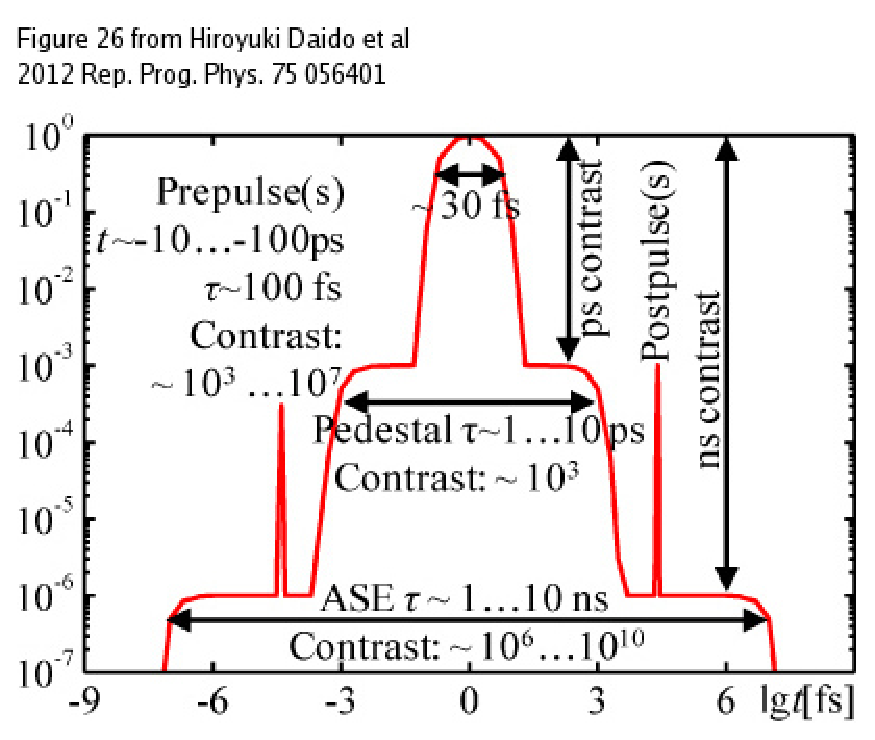
\includegraphics[width=\MyFactor\textwidth]{Img/prepulse2012.eps}
  \caption{激光脉冲示意图}
  \label{fig:prepulse2012}
\end{figure}

激光的相互过程中,设计到波-波、波-粒子、粒子-粒子的相互作
用,是一个多模、多粒子系统的强非线性相互作用过程。解析方法很难全面地进行研究,数值计算就是必然的选择。
数值模拟的方法在激光等离子体相互作用的领域中有重要的意义。首先,模拟工作往往具有前瞻性,许多重要的发现是建立在模拟工作的基础上,对实验提出要求与指导。由于数值模拟的灵活性,实验中难以达到的条件,可以在数值计算中进行模拟,寻找最优解决方法。同时,模拟工作可以解释实验中的新发现,全方位地对于物理过程进行剖析,有助于更好地理解实验现象。实验和模拟之间,互为依靠,相辅相承。现代数值模拟,借助与CPU以及GPU等高速计算工具,以及MPI和CUDA等优秀的计算平台,其计算功能已经相对成熟。
从模拟的算法角度,对于不同对象,模拟中采用不同的数值方法。对等离子体这种呈现集体运动特性的带电粒子的复杂系统(等离子体)的数值模拟研究,一般用流体力学模拟或动理学模拟方法,以及粒子模拟的方法。


\subsection{流体力学模拟}


流体力学模拟方法从宏观统计角度研究等离子体特性,例如:温度、密度、压强等,其精度在空间上百微米量级,时间上纳秒量级。其方法,是将微观得到的吸收系数或输运系数的作为已知条件,求解流体力学方程组,得到粒子的分布信息。通过粒子分布函数对参量进行积分,得到统计意义上的结果。
完整的流体力学方程组,可以通过取 Vlasov 方程的不同的速度矩得到:

连续性方程:$\partial{n_j}/\partial{t}+\partial{(n_j \bar{\vec{u_j}})}/\partial{\vec{x}} =0$


运动方程:$n_j \partial {\vec{u}_j}/\partial{t}+n \vec{u}_j \partial{\vec{u}_j}/\partial{\vec{x}} = \frac{n_j q_j}{m_j} ( \vec{E}+\frac{\vec{u}_j \times \vec{B}}{c}) - \frac{1}{m_j} \frac{\partial{\vec{p}_j}}{\vec{x}}$

状态方程:
\begin{equation}
  \begin{cases}
    p_j=n_j T_j & : \omega / k \ll v_j\\
    \frac{p_j}{{n_j}^{\gamma}}=const & : \omega / k \gg v_j
  \end{cases}
\end{equation}



其中,j代表粒子种类,温度$T_j$,热速度$v_j=(T_j/m_j)^{1/2}$,热压$P_j$。
$\gamma=(2+N)/N$,N是自由度。加上maxwell方程,以上构成流体力学的完备描述。当 $\omega / k \ll v_j$时,系统服从等温分布,当 $\omega / k \gg v_j$时,系统服从绝热分布。当 $\omega / k = v_j$时,状态方程无法描述热传递过程,需要使用Vlasov方程。因此流体力学的描述方法,适用于热传输速度远大于或者小于系统的变化速率,对于二者相当的情况,其状态方程无法用绝热或者热平衡来近似,因此流体力学方法失效。

\subsection{动力学模拟}


动力学模拟在微观上研究等离子体中的物理过程,考虑粒子在电磁场作用下运动。由于微观系统较大的复杂度,其研究等离子体的空间范围和时间尺度都有限,多用于微型空间中的快速过程。主要
包括两种方法:
(1) 求解动力学方程:
Vlasov 方程:

j类粒子在相空间随时间的分布函数 $f_j(\vec{x},\vec{v},t)$满足:
\begin{equation}
\frac{\partial{f_i}}{\partial{t}} + \vec{v} \cdot \frac{\partial{f_i}}{\partial{\vec{x}}} + \frac{1_j}{m_j}(\vec{E}+\frac{1}{c} \vec{v} \times \vec{B}) \cdot \frac{f_i}{\vec{v}}=0
\end{equation}
它描述高温无碰撞等离子体,如受控热核反应和激光等离子体相互作用。




Fokker-Plank 方程:
描述驰予扩散等非平衡状态的等离子体,在 Vlasov 方程中,加了碰撞项
$\frac{\partial{f_i}}{\partial{t}} + \vec{v} \cdot \frac{\partial{f_i}}{\partial{\vec{x}}} + \frac{1_j}{m_j}(\vec{E}+\frac{1}{c} \vec{v} \times \vec{B}) \cdot \frac{f_i}{\vec{v}}=(\partial{f}/\partial{t})_{collision}$

\begin{equation}
\label{eqn:energyCon}
\rho D_t e = -P \nabla \cdot \bf{v} - \nabla \cdot \bf{q} -Q +S
\end{equation} 

利用流体力学方程或动力学方程求解问题时,由于存在一个多维相空间的分
布函数,数值求解时要进行离散化处理,容易产生非物理的多束流失真。因此无
论是流体力学方程还是动力学方程,都需要对作为统计系统的等离子体做
平滑处理,而系统固有的统计起伏信息丢失,然而这些起伏效应在一定条件下可以发
展成象湍流这样的重要物理现象。



\section{粒子模拟}



等离子体的粒子模拟方法(PIC)起源于上世纪60年代,经过几十年的发展,其功能不断地完善,成为等离子体作用研究中的一种成熟的数值模拟方法。其原理是跟踪计算大量的粒子在自洽场以及外加磁场中的运动,运用统计平均的方法得到电流,密度等宏观量的以及等离子体中的集体效应。粒子模拟方法是从微观角度研究等离子体特性,其适用于小尺寸(例如几百电子Debye 波长)超快(几百电子等离子体频率)过程。 首先介绍PIC中的量纲,计算机模拟过程中,有些物理量非常小,如电子质量、电量、波长等,而有
些量却很大,如光速等,用计算机直接进行这些量之间的加减乘除等计算,非常
不方便,而且很有可能在计算中因变量太大而导致数值溢出或变量太小而导致有
效数字的损失。处于计算方便的考虑,物理量都做了归一化,所以在数值计算中各物理量均采用无量纲量形式:


  $t=t_{phy}/{{\omega}_{pe}}^{-1}$
  
  $x=x_{phy}/ {\lambda}_{D}$
  
  $m=m_{phy}/m_e$

  $q=q_{phy}/e$

  $n=n_{phy}/n_pe$

  $v=v_{real}/{v_{th}}$
  
  $P=\gamma mv =P_{phy}/{m_e v_{th}}$
  
  $E=E_{phy}/(m_e v_{th} \omega_{pe} /e )$
  
  $B=B_{phy}/(m_e v_{th} \omega_{pe} /e )$
  
  $J=J_{real}/(ev_{th}n_c)$
  

  
其中, $\omega_{pe}$是初始等离子体频率, $v_{th}=(k_B T_e / m_e)^{1/2}$ 是电子初始热速度, $\lambda_D=v_{th}/ {\omega}_p$是等离子体初始德拜长度,$m_e$是电子质量,e是电子电荷量,$\gamma$是相对论因子, $n_c$是等离子体临界密度。
  


PIC的基本算法如下:首先,初始化等离子体中粒子的位置速度信息以及外界电磁场源,在此基础上进行如下的循环:(1)由粒子位置和速度求解电荷密度分布以及电流密度分布,(2)电荷分布及电流密度分布,通过麦克斯韦分布求解格点中的电磁场分布,(3)由电磁场的分布更新粒子的电荷及电流密度分布,如图\ref{fig:Leapfrog}所示。其特点在于,使用宏粒子与粒子云的模型,对于粒子的分布进行描述。粒子之间的电磁作用,不是通过库仑作用描述,而是通过粒子电荷电流产生的自洽电磁场的作为媒介完成,这样很大程度上避免了库仑作用中无穷小距离下的发散问题。
\begin{figure}[!htbp]
  \centering
  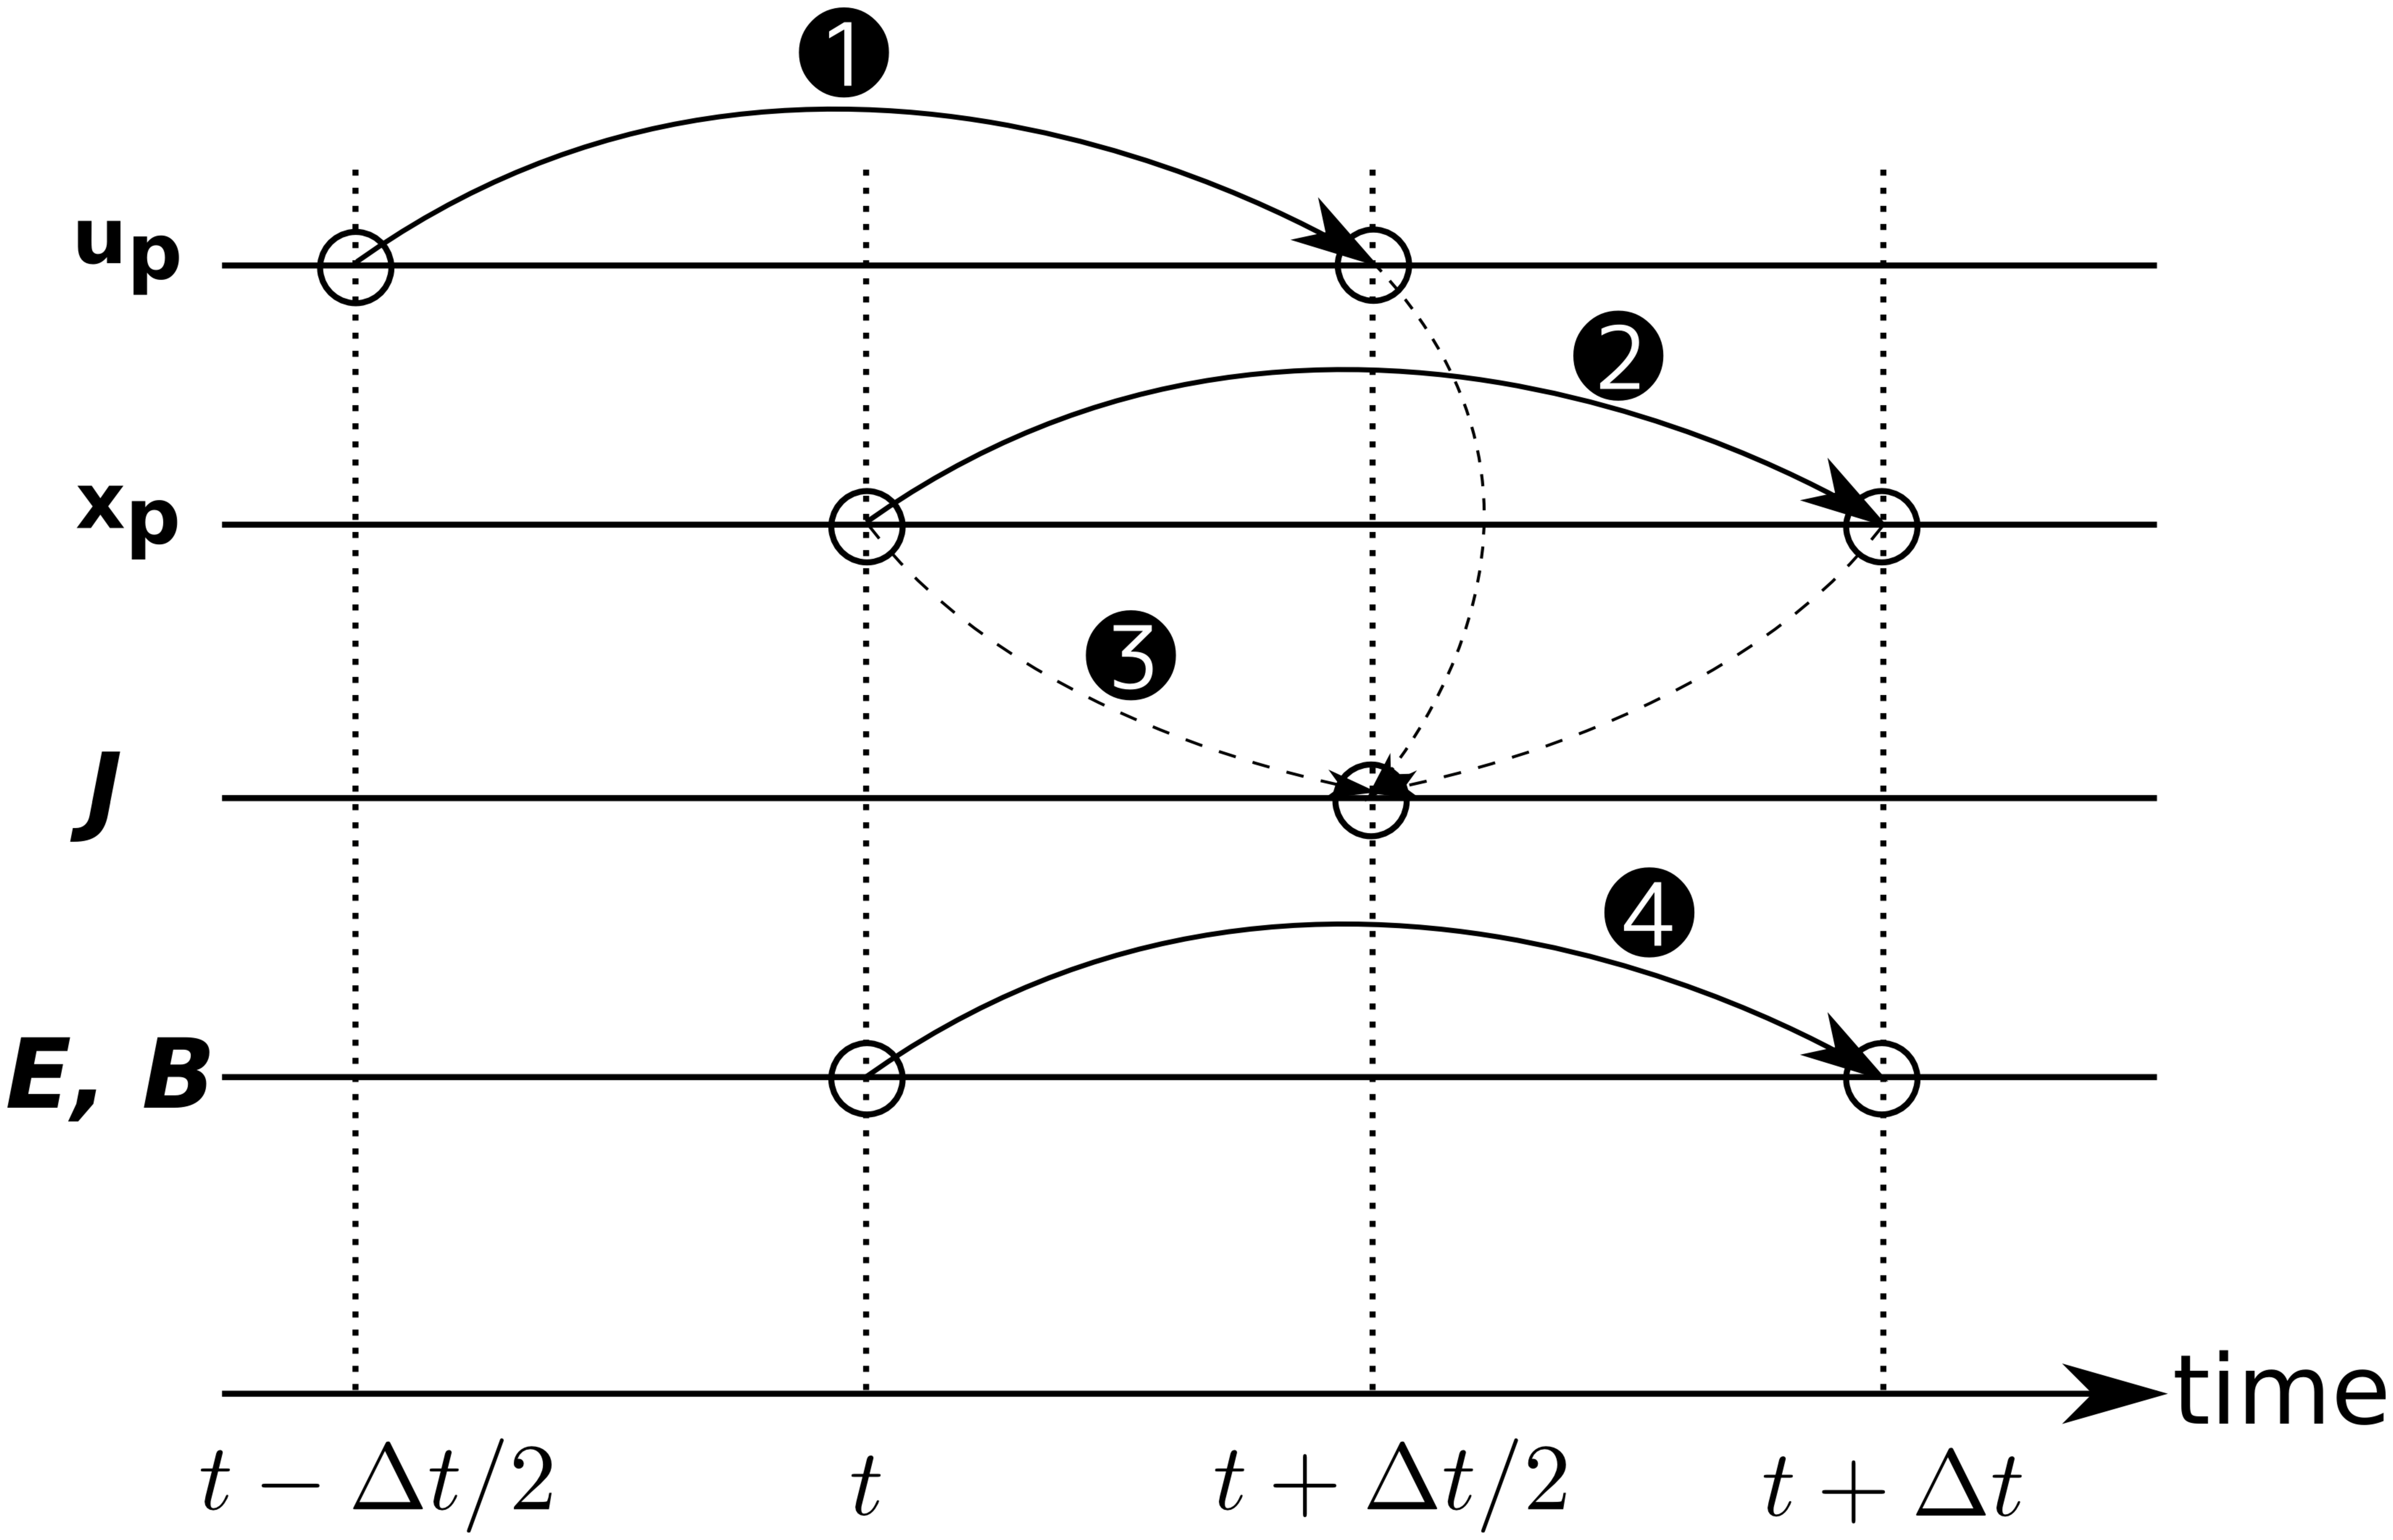
\includegraphics[width=\MyFactor\textwidth]{Img/leapfrog.eps}
  \caption{Leapfrog算法}
  \label{fig:Leapfrog}
\end{figure}

\subsection{宏粒子及粒子云模型}
实际等离子体区域中粒子数目,远远超出现有的计算机模拟能力,全部粒子模拟难度比较大。同时在等离子体分布函数的相空间
中的一点(x,v)的周围,每个带电粒子对电磁场的贡献和电磁场对粒子的作用
力都基本相同,故周围这些大量带电粒子的运动规律基本相同,因而只用一个粒
子---“粒子”代表这些粒子。对于描述等离子体中的集体效应,这种简化不会带来很大的精度上损失,也使得计算量很大程度上减少。对宏粒子系统做量纲分析


宏粒子体系中电子(代表N 个电子)的质量、电荷、温度和
密度分别为:$m^{'}=Nm$, $e^{'}=Ne$,  $n^{'}=n/N$ 。所以,

$(kT)^{'}  = m^{'}  v^{'2} = Nmv^2 = NkT$,

${{\lambda}_D}^{'} = \sqrt{ (kT)/(4 \pi n^{'} e^{'2})} = \sqrt{NkT/[4 \pi (n/N)(Ne)^2]} = \sqrt{ kT/(4 \pi ne^2 )}={{\lambda}_D}$,

$N_d=4\pi n^{'} {{\lambda}_D}^{'3}/3= 4 \pi (n/N) {{\lambda}_D}^{3} /3 = N_d/N $,

${{\lambda}_D} $ 是德拜半径,$N_d$是反映等离子体近碰撞程度的物理量,所以超粒子的引入基本上不改变等
离子体的集体效应,只是增加了粒子间近碰撞效应,引入了短波长噪声,对于超快过程(fs量级)这种碰撞效应的影响可以忽略。

宏粒子模型解决了计算量的问题,宏粒子电荷与电流对于场的影响时,存在粒子位置的问题。 由于在PIC模拟中,电磁场是以格点为存贮单元,而带点粒子在不同位置处对于格点内部电磁场的贡献是不同的,因此需要通过插值的方法,得到粒子对于其所在位置及动量状态下的电磁场的贡献。PIC中使用粒子云的方法解决这一问题的,粒子在空间中存在一定的分布,通过分布函数可以导出受力、电荷、密度等宏观属性,从而计算粒子的运动以及场的更新。一阶情况下计算粒子的电荷分布和受力插值如下:


\begin{equation}
\label{eqn:current_interpolate}
\begin{cases*}
q\vec{E}^t=q \sum_p W_p(x){\vec{E}_p}^t \\
q\vec{B}^t=q \sum_p W_p(x){\vec{B}_p}^t
\end{cases*}
\end{equation} 



其中$W_p(x)$为处于x位置的粒子在网格点$x_p$的电荷分量,即电荷分布函
数,$W_p(x)$必须满足电荷守恒,匀滑性好等特点。阶数越高,插值力越匀滑,数值噪声越小。接下来给出一个示例如何求解
1D 二阶电荷分布函数(TSC)$W_p(x)$

粒子电荷分布函数$W_p(x)$在其最邻近的三个网格点($−1$, 0,1)可以写成二
次方程形式:

\begin{equation}
\label{eqn:charge_distribution}
\begin{dcases*}
W_0(x)=ax^2+b \\
W_1(x)=W_{-1}(-x)=cx^2+dx=e
\end{dcases*}
\end{equation} 

其中粒子的位置x计算为拉格朗日步长,其定义域为$-1/2<x<1/2$。为计
算方程组\ref{eqn:charge_distribution}的待定系数,考虑粒子处于特殊位置x = 1/ 2,则有:

\begin{equation}
\begin{cases*}
W_0(1/2)=1/2  \\
W_1(1/2)=1/2  \\
W_(-1)(1/2)=0 \\
\frac{d}{dx} W_{-1}(1/2)=0  \\
\frac{d}{dx} W_{1}(1/2)=-\frac{d}{dx} W_{0}(1/2)  \\
\end{cases*}
\end{equation} 



\begin{equation}
\begin{cases*}
a=-1    \\
b=3/4  \\
c=1/2  \\
d=1/2  \\
e=1/8  \\
\end{cases*}
\end{equation} 

所以粒子电荷分布函数$W_p(x)$可以写成:

\begin{equation}
\begin{cases*}
W_0(x)=-x^2+3/4    \\
W_1(x)=W_{-1}(-x)=(x+1/2)^2/2
\end{cases*}
\end{equation}




根据位移不变性原理,$W_p(x)$也可以重写为:

\begin{equation}
 W(x) =
  \begin{cases}
   3/4-x^2 & \text{if } (|x| \leq 1/2) \\
   (3/2-|x|)^2/2 & \text{if } (1/2 \leq |x| \leq 3/2) \\
    0 & \text{其他}
  \end{cases}
\end{equation}


\begin{figure}[!htbp]
  \centering
  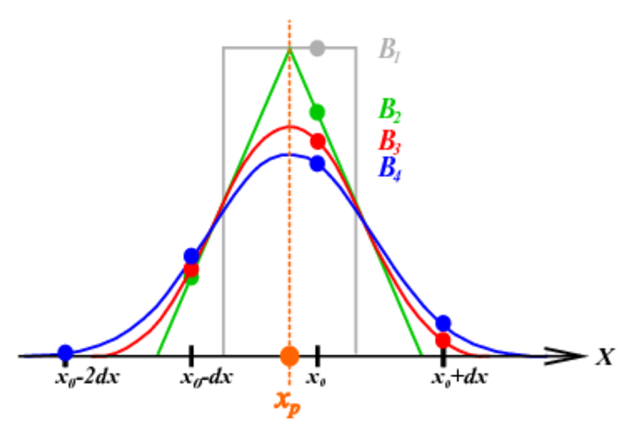
\includegraphics[width=\MyFactor\textwidth]{Img/particlecloud.eps}
  \caption{各阶贝塞尔函数粒子云分布}
  \label{fig:particlecloud}
\end{figure}
其他任意阶的电荷分布函数$W_p(x)$可以通过同样的方法计算。
将1D 的$W_p(x)$扩展为2D或3D的形式,假设各个维度之间相互独立,分别计算各维度上
粒子的电荷分布函数,然后对各维度的电荷分量函数相乘即得
到最终的电荷分布。以2D TSC 分布函数为例,每个计算粒子的电荷将分布在
其最邻近的$3^2=9$个网格点上,假设$W_i$和$W_j$分别为粒子在x和y方向上最邻近
三个网格点的电荷分布,则2D 电荷分布函数可以写成:
\begin{equation}
W_{ij}=W_{i}W_{j}
\end{equation}


粒子云的方法有效地解决了带电点粒子作用过程中距离无穷小的发散问题,通过分布函数来抑制噪声,使得计算结果尽可能的趋于实际的等离子体过程。不同的云分布对应于不同的物理模型,根据计算中的实际需求选择不同的模型。例如,对于高密度分布的等离子体,单位格点内部的粒子数目较多,低阶分布函数容易造成较大的计算噪声,高阶分布对于计算量要求较高。在保证计算精度的基础上,选择合适的分布函数。




\subsection{电磁场求解} 
电磁场的求解,是通过求解麦克斯韦方程,得到由粒子电荷以及电流产生自洽场。麦克斯韦方程的求解算法,有限时域差分法(FDTD)\cite{yee1966numerical,taflove1980application}是比较成熟且常用的。FDTD算法常采用YEE氏晶格\cite{yee1966numerical}分配电场和磁场在网格上的位置,如图\ref{fig:yee}所示。这是一种基于格点的电磁场数值计算方法,使用中心差分的方法将麦克斯韦方程差分化,使得每个格点中的电磁场只与自己相邻格点相关。基于时间空间偏微分形式的麦克斯韦方程,被差分化之后,在时间上通过电场磁场交替更新的方式演绎电磁场的时间演化过程。空间中的电场先计算,而后基于电场结果计算磁场,此过程循环往复。

无量纲化的微观麦克斯韦方程组(安培方程及法拉第方程)可以写为:  
\begin{equation}
\label{eqn:maxwell}
\begin{dcases*}
\frac{\partial{\vec{E}}}{\partial{t}} = \vec{\nabla} \times \vec{B} - 2 \pi \vec{J}  \\
\frac{\partial{\vec{B}}}{\partial{t}} = -\vec{\nabla} \times \vec{E}
\end{dcases*}
\end{equation}  
对安培方程求梯度,得到:  
${\nabla} \cdot {\partial}_t \vec{E} = c {\nabla} \cdot ({\nabla} \times \vec{B})-{\nabla} \cdot \vec{J}={\nabla} \cdot \vec{J} $, 在电荷守恒${\partial}_t  \rho + {\nabla} \cdot \vec{J} =0 $的条件下, 因此有高斯方程${\nabla} \cdot \vec{E}=\rho $恒成立。同时,如果初始条件有$\vec{\nabla} \cdot \vec{B}_{t=0}=0$, 那么由$\nabla \cdot {\partial}_t \vec{B} = -\vec{\nabla} \cdot \vec{\nabla} \times \vec{E} =0$,得到$\vec{\nabla} \cdot \vec{B}=0$恒成立。



将方程组\ref{eqn:maxwell}的矢量参数转化成标量参数,可得:
\begin{equation}
\label{eqn:maxwell_scale}
\begin{dcases*}
\partial_t {E_x}=(\partial_y {B_z} - \partial_z {B_y}) - 2 \pi J_x  \\
\partial_t {E_y}=(\partial_z {B_x} - \partial_x {B_z}) - 2 \pi J_y  \\ 
\partial_t {E_z}=(\partial_x {B_y} - \partial_y {B_z}) - 2 \pi J_z  \\
\partial_t {B_x}=(\partial_y {E_z} - \partial_z {E_y})  \\
\partial_t {B_y}=(\partial_z {E_x} - \partial_x {E_z})  \\
\partial_t {B_z}=(\partial_x {E_y} - \partial_y {E_x})
\end{dcases*}
\end{equation} 
  


%%% we need to get the graphic for the yee grid
方程\ref{eqn:YEE}为基于YEE 氏晶格将微分方程组\ref{eqn:maxwell_scale}的第一个方程转换成
差分方程的形式,其他微分方程方程也可很容易地类似写成相应的差分形式。
基于YEE氏晶格法的FDTD算法在时间和空间上都是中心差分,二阶精度。


\begin{equation}
\label{eqn:YEE}
\frac{{E_x}^{n}(i+\frac{1}{2},j,k)-{E_x}^{n-1}(i+\frac{1}{2},j,k) }{\delta t}=  \\ \frac{{B_z}^{n-\frac{1}{2}}(i+\frac{1}{2},j+\frac{1}{2},k)-{B_z}^{n-\frac{1}{2}}(i+\frac{1}{2},j-\frac{1}{2},k) }{\delta y} -  \\
\frac{{B_y}^{n-\frac{1}{2}}(i+\frac{1}{2},j,k+\frac{1}{2})-{B_y}^{n-\frac{1}{2}}(i+\frac{1}{2},j,k-\frac{1}{2}) }{\delta z}-   \\
2 \pi {J_x}^{n-1/2}(i+\frac{1}{2},j,k)
\end{equation} 





实际处理中,综合考虑计算精度计算量等,可以进行一定的简化处理,将三维程序简化为一维 、二维、
还有1D2V(一个空间分量,两个速度分量)、1D3V(一个空间分量,三个
速度分量)和2D3V(两个空间分量,三个速度分量),从而在保证研究问题的需求精度的基础上大幅度地简化计算的规模。由于本论文的工作大多基于2D3V,因此对于麦克斯韦方程的二维差分形式做以介绍。二维模型中,电磁场存在两种模式,分别是TM和TE:

\begin{figure}[!htbp]
  \centering
  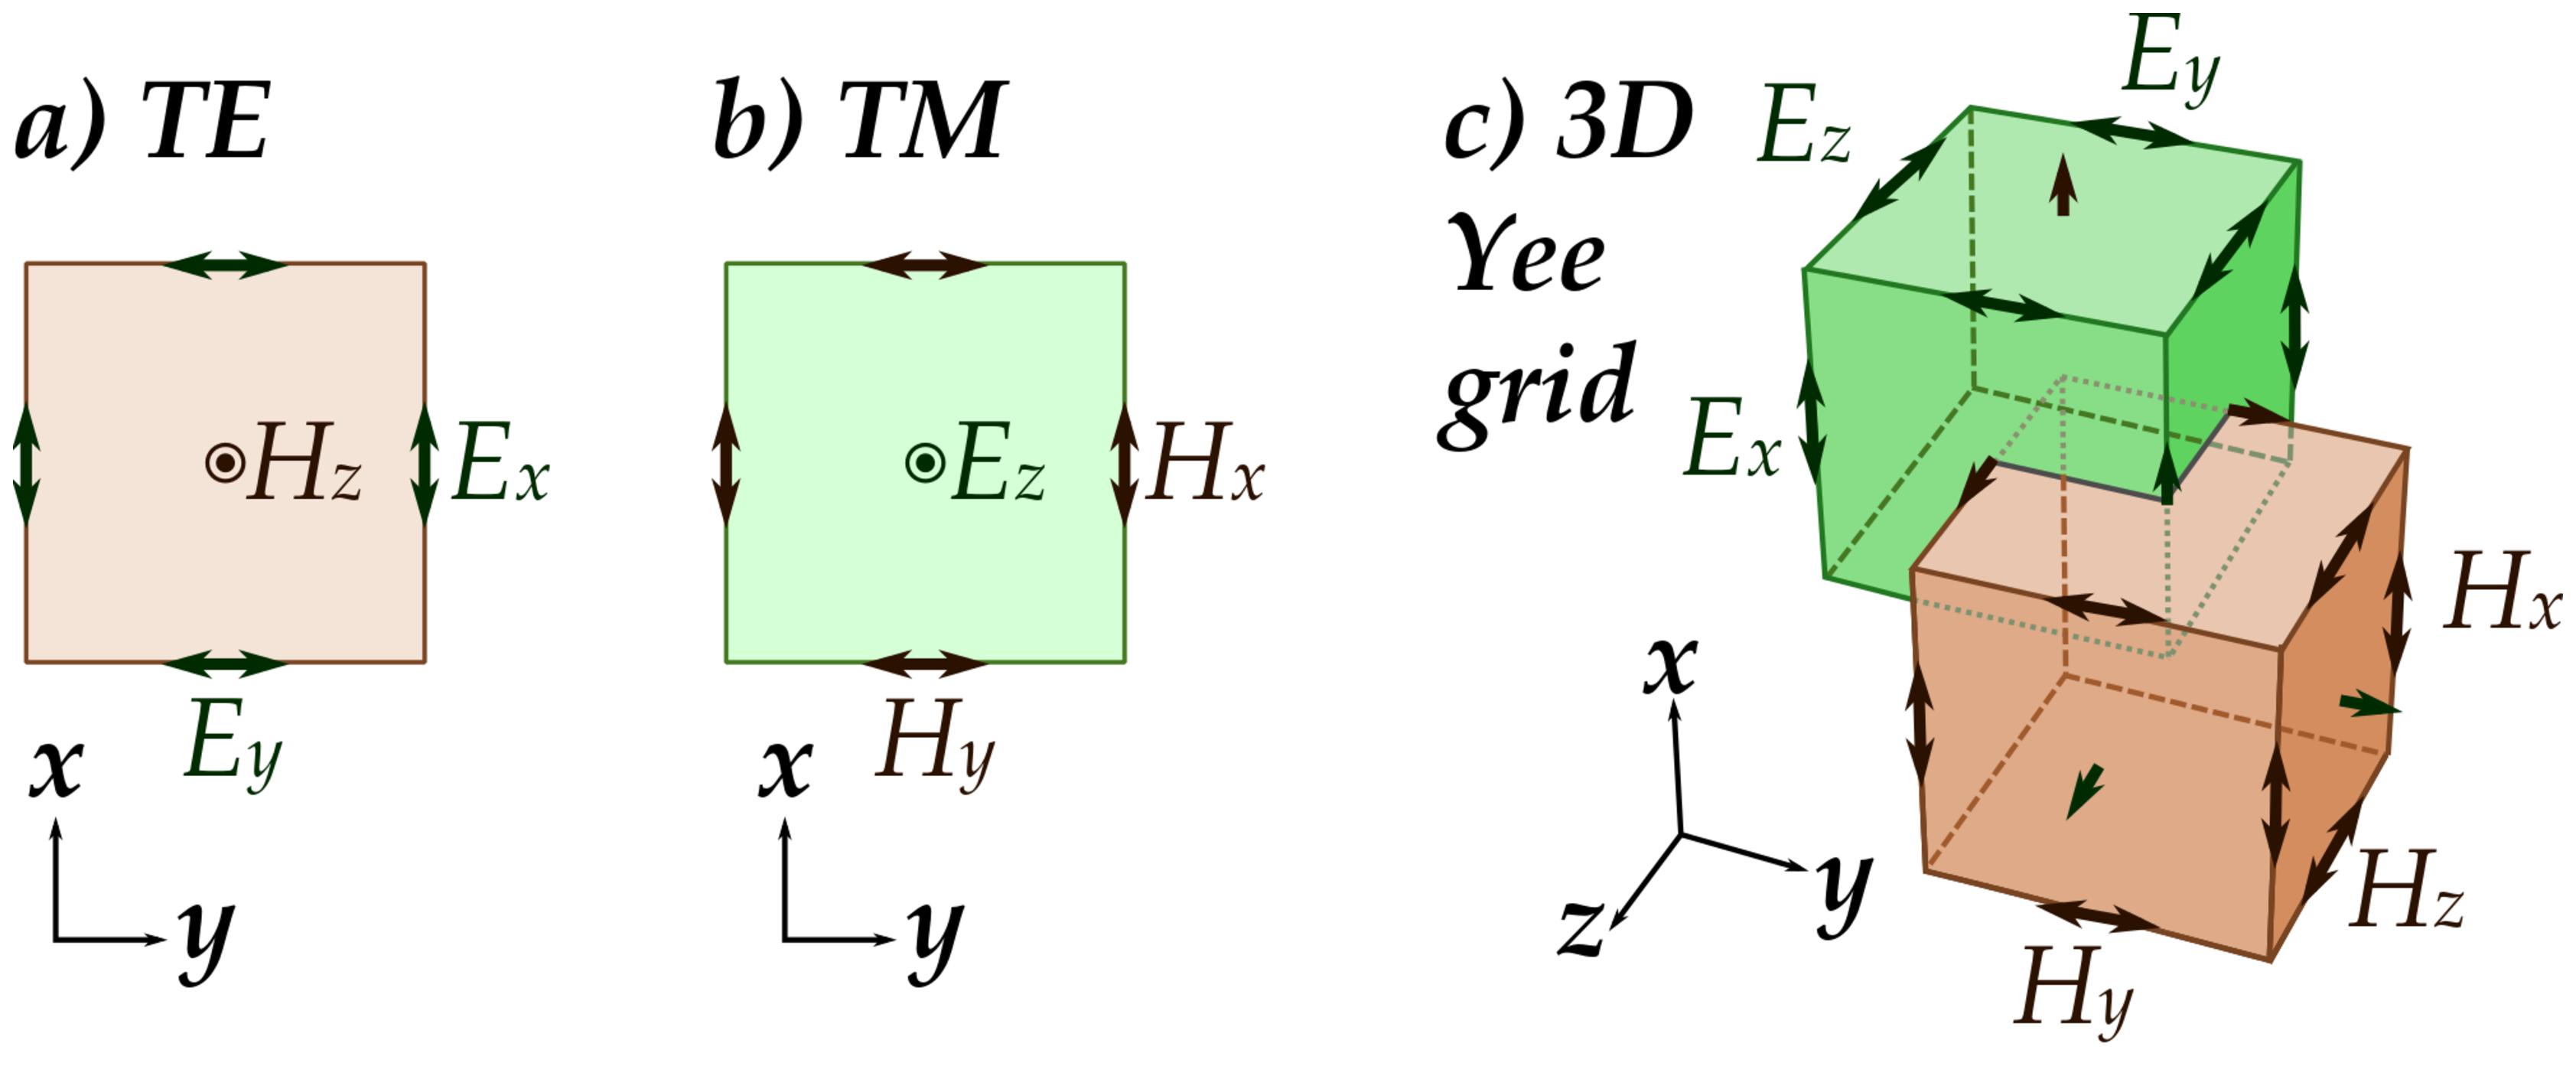
\includegraphics[width=\MyFactor\textwidth]{Img/Yee2D.eps}
  \caption{YEE氏晶格}
  \label{fig:yee}
\end{figure}



对于TM模,Maxwell方程组的二维中心差分形式

\begin{equation}
\label{eqn:maxwell_TM}
\begin{dcases*}
\frac{ {E_x}^{n+1}(i,j+1/2)-{E_x}^{n}(i,j+1/2)}{\delta t} = \frac{ {B_z}^{n+1/2}(i,j+1)-{B_z}^{n+1/2}(i,j)}{\delta y} \\
-2 \pi {J_x}^{n+1/2}(i,j+1/2)  \\
\frac{ {E_y}^{n+1}(i,j+1/2)-{E_y}^{n}(i,j+1/2)}{\delta t} = \frac{ {B_z}^{n+1/2}(i,j+1)-{B_z}^{n+1/2}(i,j)}{\delta x}  \\
-2 \pi {J_y}^{n+1/2}(i+1/2,j)  \\
\frac{ {B_z}^{n+1/2}(i,j)-{B_z}^{n-1/2}(i,j)}{\delta t} = \frac{ {E_y}^{n}(i+1/2,j)-{E_y}^{n}(i-1/2,j)}{\delta x}-   \\
\frac{ {E_x}^{n}(i,j+1/2)-{E_x}^{n}(i,j-1/2)}{\delta y}
\end{dcases*}
\end{equation} 


对于TE模,Maxwell方程组的二维中心差分形式是:

\begin{equation}
\label{eqn:maxwell_TE}
\begin{dcases*}
\frac{ {E_z}^{n+1}(i+1/2,j+1/2)-{E_z}^{n}(i+1/2,j+1/2)}{\delta t} =   \\
\frac{ {B_y}^{n+1/2}(i+1,j+1/2)-{B_y}^{n+1/2}(i,j+1/2)}{\delta x}-\frac{ {B_x}^{n+1/2}(i+1/2,j+1)-{B_x}^{n+1/2}(i+1/2,j)}{\delta x}-   \\
2 \pi {J_z}^{n+1/2}(i+1/2,j+1/2)    \\
\frac{ {B_x}^{n+1/2}(i+1/2,j)-{B_x}^{n-1/2}(i+1/2,j)}{\delta t} = \frac{ {E_z}^{n}(i+1/2,j+1/2)-{E_z}^{n}(i+1/2,j-1/2)}{\delta y}  \\
\frac{ {B_y}^{n+1/2}(i,j+1/2)-{B_y}^{n-1/2}(i,j+1/2)}{\delta t} = \frac{ {E_z}^{n}(i+1/2,j+1/2)-{E_z}^{n}(i+1/2,j-1/2)}{\delta x}
\end{dcases*}
\end{equation} 




其中空间步长$\delta x=\delta y=\delta$,时间步长$\delta t= \delta /2$,时间步长和空间步长应满足courant
条件:$(c \delta t)^2 [1/(\delta x)^2 + 1/(\delta x)^2] < 1$。


\subsection{粒子运动的求解}

%%%%%%%%%%%%%%%  we need to add the citation to 
%%%%%%% J. P. Boris, in Proceedings of the 4th Conference on Numerical Simulation of Plasma.
%%%%%%% Plasmas (Naval Res. Lab, Washington, D.C., 1970),pp. 3.
粒子运动的求解和麦克斯韦场的求解交替进行的。粒子的运动改变场分布,场信息的更新进一步促使粒子运动。PIC中使用半加速-旋转-半加速方法\cite{boris1970relativistic}解相对论粒子运动方程
   
\begin{equation}
\label{eqn:PIC_motion}
m \frac{d \vec{u}}{dt}=2 \pi q (\vec{E} + \frac{\vec{u}}{\gamma} \times \vec{B}) \\
\frac{d \vec{r}}{dt}= \vec{v}
\end{equation} 


其中$\vec{u}=\gamma \vec{v} = \vec{v}/\sqrt{1+ {{v}}^2}$,$\gamma$是粒子的相对论因子。将运动方程化成差分形式


\begin{equation}
\label{eqn:PIC_motion_derivative}
\begin{dcases*}
\frac{\vec{u}^{n+1/2}-\vec{u}^{n-1/2}}{dt}=\frac{2 \pi q }{m} (\vec{E}^n + \frac{\vec{u}^{n+1/2}+\vec{u}^{n-1/2}}{2\gamma} \times \vec{B}^n)  \\
\frac{\vec{r}^{n}-\vec{r}^{n-1}}{dt}= \vec{v}^{n+1/2}
\end{dcases*}
\end{equation} 


做如下替换
\begin{equation}
\label{eqn:PIC_half_acceleration}
\begin{dcases*}
\vec{u}^{n-1/2} = \vec{u}^{-}- \frac{\pi q }{m} \vec{E}^n \delta t   \\
\vec{u}^{n+1/2} = \vec{u}^{+} +\frac{\pi q }{m} \vec{E}^n \delta t
\end{dcases*}
\end{equation} 

,上式转化为
\begin{equation}
\label{eqn:PIC_half_acceleration}
\begin{dcases*}
{\vec{u}^{+}-\vec{u}^{-}}=\frac{2 \pi q }{m} \frac{{\delta} t}{2 {\gamma}^n} (
{\vec{u}^{+} + \vec{u}^{-}}) \times \vec{B}^n)
\end{dcases*}
\end{equation} 


进一步,$\vec{t}= \frac{2 \pi q}{m} \frac{{\delta} t}{2 {\gamma}^n} \vec{B}^n$,$\vec{s}=\frac{2\vec{t}}{1+t^2}$,可得


\begin{equation}
\label{eqn:PIC_half_acceleration1}
\begin{dcases*}
\vec{u}^{'}=\vec{u}^{-} + \vec{u}^{-} \times \vec{t}   \\
\vec{u}^{+}=\vec{u}^{-} + \vec{u}^{'} \times \vec{s}
\end{dcases*}
\end{equation} 


其基本步骤如下所示:

\begin{equation}
\label{eqn:PIC_half_explain}
 \vec{u}^{n-1/2} \xrightharpoondown[在前\delta/2时间内]{\vec{E}^n 作用,加速} \vec{u}^{-} \xrightharpoondown[]{\vec{B}^n 作用,旋转} \vec{u}^{+} \xrightharpoondown[在后{delta t}/2时间内]{\vec{E}^n 作用,加速} I \vec{u}^{n+1/2} 
\end{equation}


\begin{figure}[!htbp]
  \centering
  \includegraphics[width=\MyFactor\textwidth]{Img/Boris.eps}
  \caption{Boris半加速半旋转方法}
  \label{fig:Boris}
\end{figure}

   




   
 



\subsection{电流密度计算}

由连续方程${\partial}_t \rho = - \vec{\nabla} \cdot \vec{J}$可知,带电计算粒子的运动会产生电流,电流又产生相应的电磁场。在数值计算粒子运动方程中,所得的粒子速度有一定的误差,所以由
简单的面积平均法求解电流密度分布$\vec{J}=en\vec{v}$并不能严格满足连续方程,
而需求解泊松方程对电场进行修正\cite{hockney1988computer},这需要长程计算,并不易于并行优
化。但若计算该局部电流的过程中满足电荷守恒的条件,则可以避免求解泊松
方程。由连续方程可知,电流密度可由粒子的电荷密度分布变化表征。在
PIC 模拟中,计算粒子并非一个质点,而可以定义为其宏观属性如电荷,密
度,产生的电流等在网格格点上的分布,该分布取决于给定的插值函数和粒子
的位置,而与粒子速度无关。所以局部电流密度的计算将变得非常简单: 只需求
解计算粒子在其附近网格格点上前后时刻的电荷密度分量,再由各格点的电荷
密度变化率即可得该格点的电流密度。假设某粒子$t_0$和$t_1$时刻在其附近网格点
的电荷密度分布分别为矩阵$W_0$和$W_1$,则各网格点的电荷密度变化为:


\begin{equation}
T=W_1-W_0
\end{equation}

则对应产生的电流密度变化$\delta J$为:

\begin{equation}
\delta J =\frac{q}{V} \frac{\delta x}{\delta t} T = \frac{q}{V} \frac{\delta x}{\delta t}(W_1-W_0)
\end{equation}


值得注意的是,为抑制数值加热,电荷密度分布的变化必须很匀滑,因此可以采用高阶分布函数。在电荷
守恒的条件下,J. Villasenor 和O. Buneman 给出了基于一阶电荷分布CIC的电
流密度计算方法\cite{villasenor1992rigorous},但因考虑到各种边界情形,其计算形式非常复杂。而后T.
Z. Esirkepov 给出了任意阶电荷分布函数下电流密度计算的统一形式\cite{esirkepov2001exact},该形
式可以直接用于PIC中。



\section{结论}

随着计算工具和计算方法的发展,PIC本身也有重要的进步。不同版本的程序相继出现,且其功能已经从最初的简单的模型扩展到更全面的等离子体模拟,包括电离、碰撞、辐射等热门应用领域,且在不断地完善。与此同时计算方法以及平台也在相继进步。例如,电磁场的计算中,出现了例如Direct Spliting\cite{sentoku2008numerical}等方法,相对于成熟的有限时域差分方法,具有速度与精度的双重优势,缺点是无法模拟激光斜向入射的情况。德国HZDR的激光加速模拟小组,开展了将PIC发展到GPU上的工作,取得了重要的突破。利用性能优越的商业化GPU硬件以及成熟的并行化编程平台CUDA,使得PIC计算速度相对于传统的CPU服务器,其速度提高了将近20倍以上,这在计算等离子体领域是一个很重要的进步。



